\documentclass[11pt, letterpaper]{article}
\usepackage[utf8]{inputenc}
\usepackage[margin=1in]{geometry}
\usepackage{enumitem}
\usepackage{indentfirst}
\usepackage{titling}
\usepackage{graphicx}
\usepackage{amsmath}
\usepackage{mathtools}
\usepackage{hyperref}
\usepackage{mathabx}
\usepackage{caption}
\usepackage{subcaption}
\usepackage{bm}
\usepackage{textcomp}
\graphicspath{ {./} }
\DeclareMathAlphabet{\altmathcal}{OMS}{cmsy}{m}{n}

\newcommand{\bv}[2][]{\bm{\vec{#2}_{#1}}}

\setlength{\parindent}{0cm}
\setlength{\parskip}{1em}
\renewcommand{\baselinestretch}{1.5}

\hypersetup{
    colorlinks=true,
    linkcolor=cyan,
    filecolor=magenta,      
    urlcolor=blue,
}

\title{Chapter V: Circuits}
\author{Chenyi Zhu}
\date{March 20th, 2020}

\begin{document}


\begin{titlingpage}
	\maketitle
	
	\begin{center}
		``Apply Kirchoff's Law, they said.''
	\end{center}
	
	\begin{figure}[h!]
		\centering
		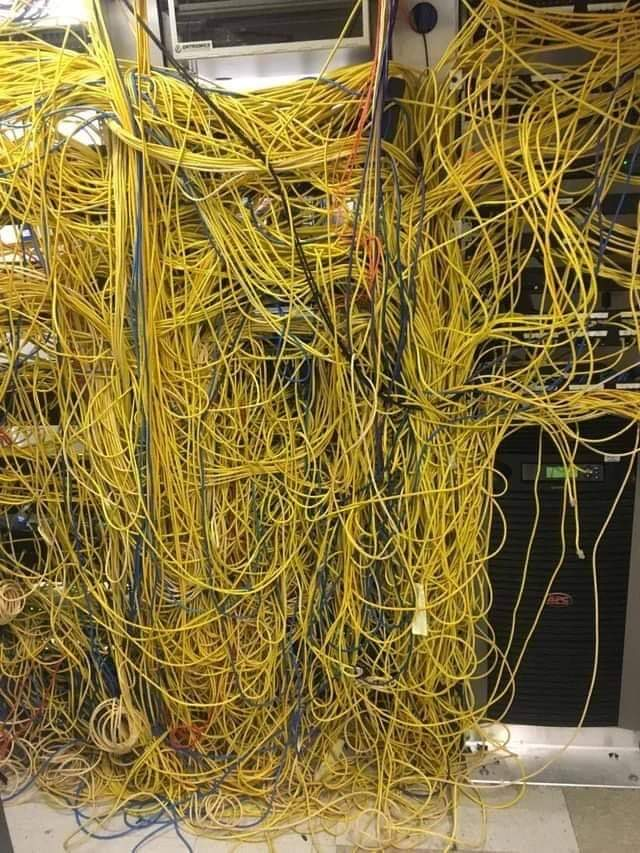
\includegraphics[scale=0.4]{loops}
		\label{fig:flux}
	\end{figure}
		
\end{titlingpage}
	
\section{Electric Current.}
	We use \textbf{current} to describe the flow of charge.
	\begin{figure}[h!]
		\centering
		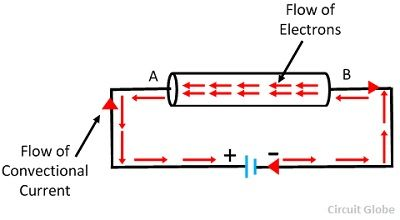
\includegraphics[scale=0.5]{current.jpg}
		\caption{Flow of electrons.}
		\label{fig:current}
	\end{figure}
	
	The electric current is defined as the flow rate of charges across a cross-sectional area. If an amount of charge $\Delta Q$ passes through a surface over period $\Delta t$, then the average current $I_{avg}$ is defined as: \[I_{avg} = \frac{\Delta Q}{\Delta t}\] whose SI unit is ampere ($A$), and $1\, A = 1\, C/s$. Take $\lim_{t\to 0}$ we obtain the instantaneous current $I$: 
\begin{equation}\label{eqn:curr}
	\boxed{I = \frac{dQ}{dt}}
\end{equation}
Flow has a direction, so we introduce the convention that the direction of current corresponds to the direction in which positive charges are flowing. In reality, we have negatively charged electrons which flow in the opposite direction of current as we define it.

\textbf{Note}: Electric currents flow in conductors: solids, liquids, or gasses, but are impeded in insulators.

\textbf{Note}: common currents range from mega-amperes (lightening) to nano-amperes (neurons firing), so if your calculations tell you otherwise, you should check your math.

	\subsection{Current Density}
	Current is a macroscopic concept, now we need to relate the macroscopic to the microscopic (electrons flowing) phenomena.\newpage
	\begin{figure}[h!]
		\centering
		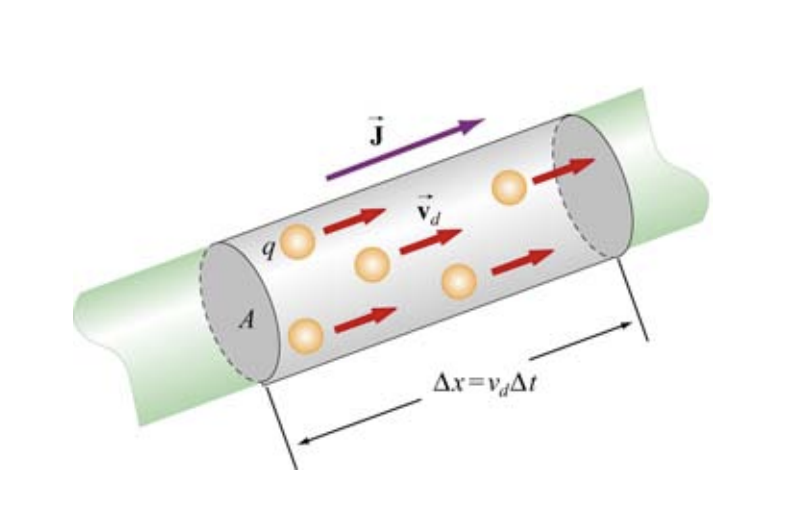
\includegraphics[scale=0.5]{curr-density.png}
		\caption{Current flowing in a conductor.}
		\label{fig:curr-density}
	\end{figure}
	Let the total current through a surface be written as: \[I = \iint\vec{\bm{J}}\cdot\, d\vec{\bm{A}}\] where $\vec{\bm{J}}$ is the current density (SI unit: $A/m^2$). If each carrier has charge $q$, and number of charge per unit volume $n$, the total amount of charge in this cross-section is $\Delta Q = q(nA\Delta x)$. Suppose that the charges move with a speed $v_d$, then the displacement in a time interval will be $\Delta x = v_d\Delta t\implies$
	\begin{equation}\label{eqn:avg-current}
		\boxed{I_{avg} = \frac{\Delta Q}{\Delta t} = nqv_dA}
	\end{equation}

$v_d$ is the \textit{drift speed} of the charge carriers, computed as the average speed of the charges inside a conductor when en external electric field is applied. As you may guess, electrons inside the conductor does not travel in straight lines, but in an erratic manner.

\begin{figure}[h!]
	\centering
	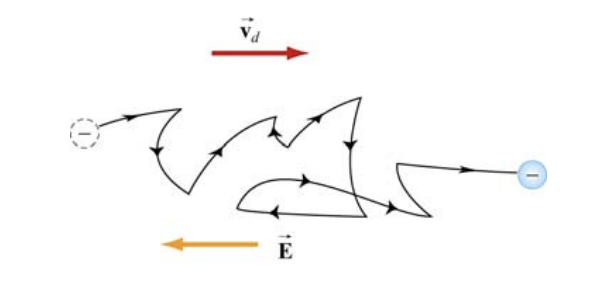
\includegraphics[scale=0.5]{drift.png}
	\caption{Motion of an electron.}
	\label{fig:drift}
\end{figure} 
From the above information, we obtain equation for $\vec{\bm{J}}$, the current density as:
\begin{equation}\label{eqn:current-density}
	\boxed{\vec{\bm{J}} = nq\bm{\vec{v}_d}}
\end{equation} 
and we have hence defined $\bv{J}$ and $\bv[d]{v}$ to have the same direction. 
\pagebreak

Then, in order to find the drift velocity of electrons, we first note that an electron inside the conductor will experience a force $\bv[e]{F} = -e\bv{E}$, from which we can derive acceleration: \[\bv{a} = \frac{\bv[e]{F}}{m_e} = -\frac{e\bv{E}}{m_e}\] Let the velocity of a given electron immediately after a collision be $\bv[i]{v}$. The velocity of the electron right before the next collision is given by: \[\bv[f]{v} = \bv[i]{v} + \bv{a} t = \bv[i]{v} - \frac{e\bv{E}}{m_e} t\] where t is the time interval. The average of $\bv[f]{v}$ over all time intervals is \[\langle\bv[f]{v}\rangle = \langle\bv[i]{v}\rangle - \frac{e\bv{E}}{m_e}\langle t\rangle\] which is the drift velocity $\bv[d]{v}$ as we wanted. Looking at our initial conditions, in the absence of an electric field, the velocity of the electron would be completely random, and it would follow that $\langle\bv[i]{v}\rangle = 0$. Let $\tau = \langle t\rangle$ be the \textit{average characteristic time} between successive collisions (fancy terminology warning: also called \textit{mean free time}), rewriting the equation above gives us \[\bv[d]{v} = \langle\bv[f]{v}\rangle = -\frac{e\bv{E}}{m_e}\tau\] and current density becomes
\begin{equation}\label{eqn:curr-density}
	\boxed{\bv{J} = -ne\bv[d]{v} = -ne\left(-\frac{e\bv{E}}{m_e}\tau\right) = \frac{ne^2\tau}{m_e}\bv{E}}
\end{equation}
For consistency, note that $\bv{J}$ and $\bv{E}$ will always have the same direction.

\section{Ohm's Law.}
	There are two different versions of Ohm's Law: microscopic and macroscopic. You may be more familiar with the latter: \[\Delta V = IR\] but this can be expressed in a different but equivalent microscopic form: \[\bv{J} = \sigma\bv{E}\] Let us explore the relationships between these two forms of Ohm's Law.
	
	In many materials, the current density is linearly dependent on the external electric field $\bv{E}$ and this relation is exactly 
	\begin{equation}\label{eqn:micro-ohm}
		\boxed{\bv{J} = \sigma\bv{E}}
	\end{equation} where $\sigma$ is called the \textbf{conductivity} of the material. A material that obeys this relation is said to be  \textbf{ohmic}; otherwise the material is \textbf{non-ohmic}.
	
	Compare equations \hyperref[eqn:curr-density]{(4)} and \hyperref[eqn:micro-ohm]{(5)}, we see that conductivity can be expressed as 
	\begin{equation}\label{eqn:conductivity}
		\boxed{\sigma = \frac{ne^2\tau}{m_e}}
	\end{equation}
To obtain the macroscopic form (which is more useful for our purposes), consider a segment of straight wire of length $l$ and non-negligible cross-sectional area $A$:
\begin{figure}[h!]
	\centering
	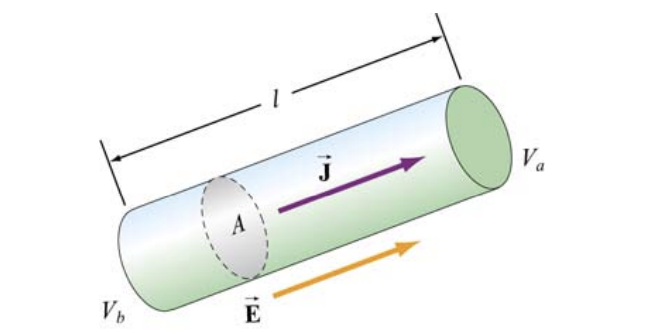
\includegraphics[scale=0.6]{wire.png}
	\caption{Uniform wire of length $l$, area $A$, and potential difference $\Delta V = V_b - V_a$.}
	\label{fig:wire}
\end{figure}

Suppose a potential difference $\Delta V = V_b - V_a$ is applied between the wire's ends, creating an electric field $\bv{E}$ and current $I$. Assuming $\bv{E}$ to be uniform, we have \[\Delta V = V_b - V_a = -\int_a^b\bv{E}\cdot\, d\bv{s} = El\] Rearrange the equation, we can rewrite current density (magnitude) as \[J = \sigma E = \sigma\left(\frac{\Delta V}{l}\right)\]. With $J = I/A$ by definition, the potential difference becomes \[\Delta V = J\frac{l}{\sigma} = \left(\frac{l}{\sigma A}\right)I = RI\] where we define \textbf{resistance} as 
\begin{equation}\label{eqn:resistance}
	\boxed{R = \frac{\Delta V}{I} = \frac{l}{\sigma A}} 
\end{equation}
and we have hence obtained the macroscopic form of Ohm's Law:
\begin{equation}\label{eqn:macro-ohm}
	\boxed{\Delta V = IR}
\end{equation}
The SI unit of resistance $R$ is the \textbf{ohm} ($\Omega$), defined as $1\,\Omega \equiv 1\,V/1\,A$. 

Again, a material that satisfies the above macroscopic Ohm's Law is ohmic, otherwise non-ohmic. Most metals (which have high conductivity and low resistivity) are considered ohmic materials. You will only work with ohmic materials, though. 
\begin{figure}[h!]
	\centering
	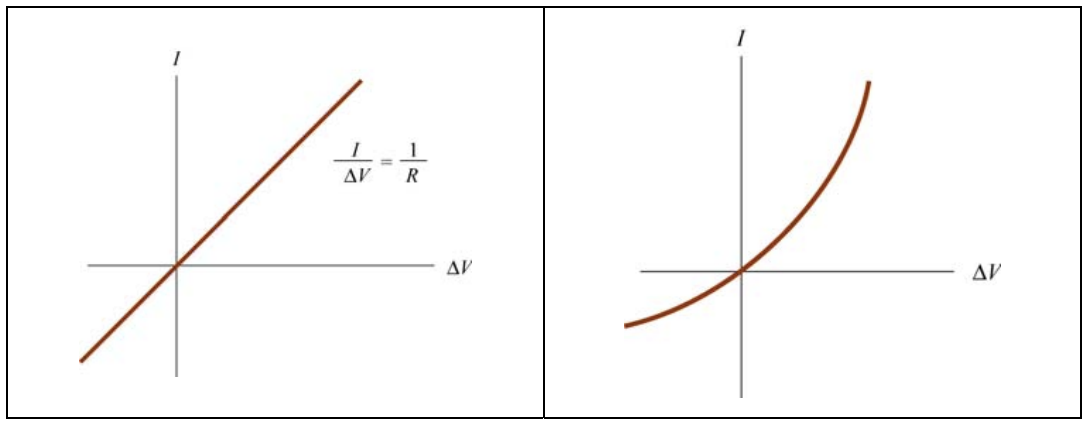
\includegraphics[scale=0.5]{ohm.png}
	\caption{Ohmic v.s. non-ohmic behaviors.}
	\label{fig:ohm}
\end{figure}

Now that we have defined conductivity, we will define \textbf{resistivity} as the inverse of conductivity:
\begin{equation}\label{eqn:resistivity}
	\boxed{\rho = \frac{1}{\sigma} = \frac{m_e}{ne^2\tau}}
\end{equation}
and we have found a new (more intuitive) way to define resistance, in terms of resistivity instead of conductivity: 
\begin{equation}\label{eqn:resist}
	\boxed{R = \frac{\rho l}{A}}
\end{equation}
\textbf{Note}: The resistivity of a material varies with temperature $T$. For metals, this variation is linear over a large range of $T$:
\begin{equation}\label{eqn:temp}
	\boxed{\rho = \rho_0[1 + \alpha(T - T_0)]}
\end{equation}
where $\alpha$ is $\textit{temperature coefficient of resistivity}$. See \hyperref[sec:app]{Appendix} of typical $\rho$, $\sigma$, and $\alpha$ (at 20\textdegree{}C) for different types of materials.
\newpage

\section{Energy and Power.}
Consider a simple circuit consisting of a battery and a resistor of resistance $R$.
\begin{figure}[h!]
	\centering
	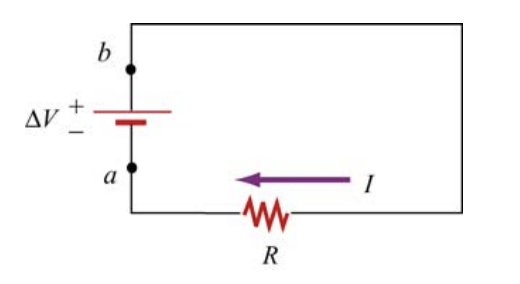
\includegraphics[scale=0.7]{circuit.png}
	\caption{Simple circuit.}
	\label{fig:circuit}
\end{figure}

Let the potential difference between two points $a$ and $b$ be $\Delta V = V_b - V_a > 0$, then if a charge $\Delta q$ is moved from $a$ to $b$ across the battery directly, then the electric potential energy would increase by $\Delta U = \Delta q\Delta V$. On the other hand, when the charge moves across the resistor in the direction of the current $I$, a loss in potential energy is incurred due to collisions with atoms in the resistor. Ignore the internal resistance of the battery and the wire itself, from the time when the charge leaves the resistor to when it arrives again at $a$, the potential energy of $\Delta q$ is unchanged. Thus, we obtain the rate of energy loss:
\begin{equation}
	\boxed{P = \frac{\Delta U}{\Delta t} = \left(\frac{\Delta q}{\Delta t}\right)\Delta V = I\Delta V}
\end{equation}
which is exactly the power supplied by the battery. Upon substitution $\Delta V = IR$, we get:
\begin{equation}
	\boxed{P = I^2R = \frac{(\Delta V)^2}{R}}
\end{equation}
\newpage

\section{Appendix}
\label{sec:app}
\subsection{Materials and Resistivity}
\begin{figure}[h!]
	\centering
	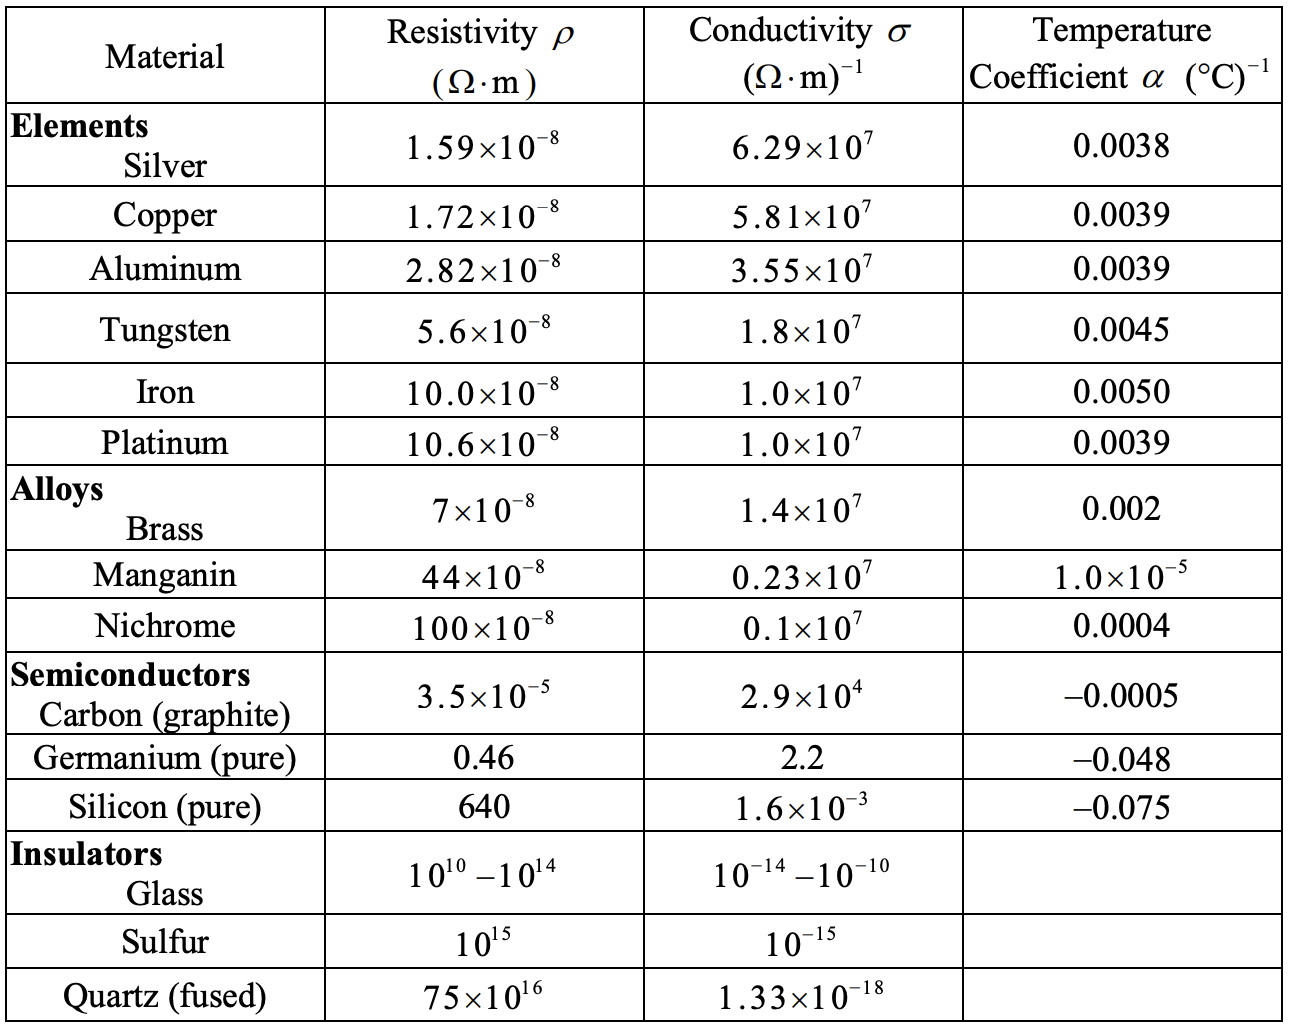
\includegraphics[scale=0.6]{resistivity.png}
\end{figure}

\newpage
\section{Exercises.}
\subsection{Warm-up}
%6.5.1
\textbf{Problem 1}. A $3000\, km$ long cable consists of seven copper wires, each of diameter $0.73\, mm$, bundled together and surrounded by an insulating sheath. Calculate the resistance of the cable (resistivity of copper: $3\cdot 10^{-6}\,\Omega\cdot cm$).

\subsection{Conceptual Questions}
%6.6
\textbf{Problem 2}. Two wires $A$ and $B$ of circular cross-section are made of the same metal and have equal lengths, but the resistance of wire $A$ is four times greater than that of wire $B$. Find the ratio of their cross-sectional areas.

\textbf{Problem 3}. From the point of view of atomic theory, explain why the resistance of a material increases as its temperature increases.

\textbf{Problem 4}. Two conductors $A$ and $B$ of the same length and radius are connected across the same potential difference. The resistance of conductor A is twice that of B. To which conductor is more power delivered?

\subsection{More Practice}
%6.5.2-4
\textbf{Probelm 5}. Show that the total amount of charge at junction of the two materials is $\varepsilon_0I(\sigma_2^{-1} - \sigma_1^{-1})$, where $I$ is the steady current flowing through the junction, and $\sigma_i$ is the conductivity of the material.\\
\textbf{Hint}: What does it mean for $I$ to be a steady current? What does that tell you about the current density $\bv{J}$?
\begin{figure}[h!]
	\centering
	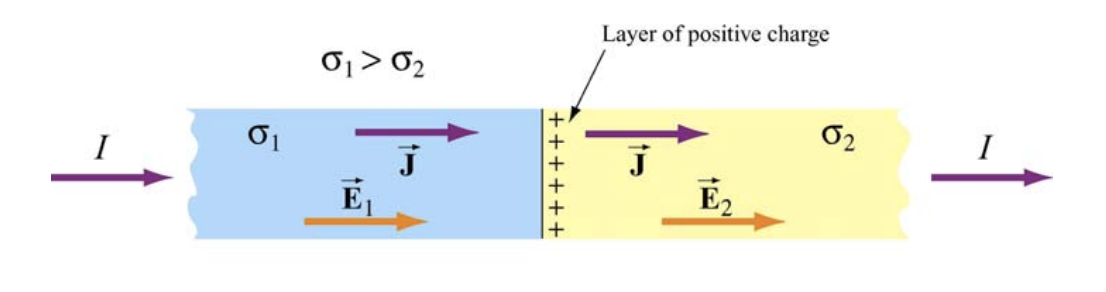
\includegraphics[scale=0.5]{junction.png}
	\caption{Two materials with different conductivities in contact.}
	\label{fig:junction}
\end{figure}

\textbf{Problem 6}. The resistivity of seawater is about $25\, \Omega\cdot cm$. The charge carriers are chiefly $Na^+$ and $Cl^-$ ions, and of each there are about $3\cdot 10^{20}/cm^3$. If we fill a plastic tube 2 meters long with seawater and connect a $12\, V$ battery to the electrodes at each end, what is the resulting average drift velocity of the ions?

\textbf{Problem 7}. Consider a material of resistivity $\rho$ in a shape of a truncated cone of altitude $h$, and radii $a$ and $b$, for the right and the left ends, respectively. Assuming that the current is distributed uniformly throughout the cross-section of the cone, what is the resistance between the two ends?
\begin{figure}[h!]
	\centering
	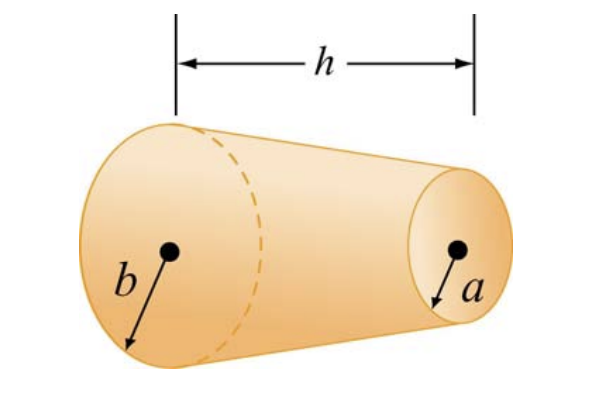
\includegraphics[scale=0.5]{trunc.png}
	\caption{Truncated cone.}
	\label{fig:truncated}
\end{figure}

\end{document}
